\chapter{Gibbs Sampling in Prob. Submodular Models} \label{ch:gibbs}

\emph{The majority of the content of this chapter has already been published in conference proceedings \citep{gotovos15}.}

\section{Introduction}
In this chapter, we consider one of the simplest and most commonly used sampling procedures, namely the (single-site) Gibbs sampler, which is also known as the Glauber chain.
While there has been extensive work on the properties of the Gibbs sampler on low-order models, for example, Ising models \citep[Ch. 15]{levin08book}, not much is known about its behavior on higher-order models, except that, in general, we cannot hope for sub-exponential mixing times \citep{jerrum93}.
In fact, we show that even for probabilistic submodular models defined by monotone submodular functions, there are simple model families with exponential lower bounds on mixing time.

Our goal is to establish theoretical conditions that guarantee rapid mixing of the Gibbs sampler in probabilistic submodular models, and at the same time, investigate in what way the properties of sub- and supermodularity affect the resulting conditions.


\section{Problem Setup} \label{sect:setup}
In this chapter, we focus on distributions of the form
\begin{align}\label{eq:pdef}
p(S) = \frac{\exp(\beta F(S))}{Z},
\end{align}
for all $S \subseteq V$, where $F$ is submodular or supermodular.
We currently assume that $F$ is already learned or given, and omit the parameter vector $\btheta$ from the notation.
Furthermore, we have introduced a scaling parameter $\beta \geq 0$, which is referred to as inverse temperature, and will be useful for our subsequent theoretical analysis.
Intuitively, $\beta$ controls the concentration of $p$ around the high-value sets of $F$.
When $\beta = 0$, $p$ is the uniform distribution over $2^V$; when $\beta \to \infty$, the mass of $p$ fully concentrates around the maximizers of $F$.


\paragraph{Marginal inference.}
Our goal is to perform marginal inference for the distributions described above.
Concretely, for some fixed $A \subseteq B \subseteq V$, we would like to compute the probability of sets $S$ that contain all elements of $A$, but no elements outside of $B$, that is, $p(A \subseteq S \subseteq B)$.
More generally, we are interested in computing conditional probabilities of the form $p(A \subseteq S \subseteq B \mid C \subseteq S \subseteq D)$.
This computation can be reduced to computing unconditional marginals as follows.
For any $C \subseteq V$, define the contraction of $F$ on $C$, $F_C : 2^{V \setminus C} \to \mathbb{R}$, by $F_C(S) = F(S \cup C) - F(S)$, for all $S \subseteq V \setminus C$.
Also, for any $D \subseteq V$, define the restriction of $F$ to $D$, $F^D : 2^D \to \mathbb{R}$, by $F^D(S) = F(S)$, for all $S \subseteq D$.
If $F$ is submodular, then its contractions and restrictions are also submodular, and, thus, $(F_C)^D$ is submodular.
Finally, it is easy to see that $p(S \mid C \subseteq S \subseteq D) \propto \exp(\beta (F_C)^D(S))$.
In our experiments, we consider computing marginals of the form $p(v \in S \mid C \subseteq S \subseteq D)$, for some $v \in V$, which correspond to $A = \{v\}$, and $B = V$.

\paragraph{The Gibbs sampler.}
We first set up some notation that is used throughout this chapter.
We denote by $\ss \defeq 2^V$ the state space, and by $P$ the transition matrix of the chain.
Each element $P(x, y)$ corresponds to the conditional probability of transitioning from state $x \in \ss$ to state $y \in \ss$, that is, $P(x, y) \defeq P(X_{t+1} = y \mid X_{t} = x)$, for any $x, y \in \ss$, and any $t \geq 0$.
We also define an adjacency relation $x \sim y$ on the elements of the state space, which denotes that $x$ and $y$ differ by exactly one element.
It follows that each $x \in \ss$ has exactly $n$ neighbors.

We define the Gibbs sampler by an iterative two-step procedure, as shown in \algoref{alg:gibbs}.
First, we select an element $v \in V$ uniformly at random; then, we add or removes $v$ to the current state $X_t$ according to the conditional probability of the resulting state.
In \figref{fig:gibbs} we illustrate one step of the Gibbs sampler on a small ground set $V = \{1, 2, 3\}$.
Assuming that the current state is $X_t = \{2\}$, there are three potential new next states, namely $\varnothing$, $\{1, 2\}$, or $\{2, 3\}$, which are the three neighbors of $X_t$ in the state space.
The Gibbs sampler first selects one of the neighbors uniformly at random, and then either stays at $X_t$ or moves to that neighbor according to the corresponding conditional probability.

\begin{algorithm}[tb]
    \setstretch{1.3}
    \DontPrintSemicolon
    \SetKwInOut{Input}{Input}
    \Input{Ground set $V$, distribution $p(S) \propto \exp(\beta F(S))$}
	$X_0$ $\gets$ random subset of $V$\\
	\For{$t = 0$ \KwTo $N_{\mathrm{iter}}$}{
	  $v$ $\gets$ $\mathrm{Unif}(V)$\;
	  $\Delta_F(v \mid X_t)$ $\gets$ $F(X_t \cup \{v\}) - F(X_t \setminus \{v\})$\;
	  $p_{\mathrm{add}}$ $\gets$ $\exp(\beta\Delta_F(v | X_t))/(1 + \exp(\beta\Delta_F(v | X_t)))$\;
	  $z$ $\gets$ $\mathrm{Unif}([0,1])$\;
	  \uIf{$z \leq p_{\mathrm{add}}$}{
        $X_{t+1} \gets X_t \cup \{v\}$\;
      } \Else{
        $X_{t+1} \gets X_t \setminus \{v\}$\;
      }
    }
    \vspace{1em}
	\caption{The Gibbs sampler for probabilistic submodular models.}
	\label{alg:gibbs}
\end{algorithm}

\begin{figure}[htb]
\centering
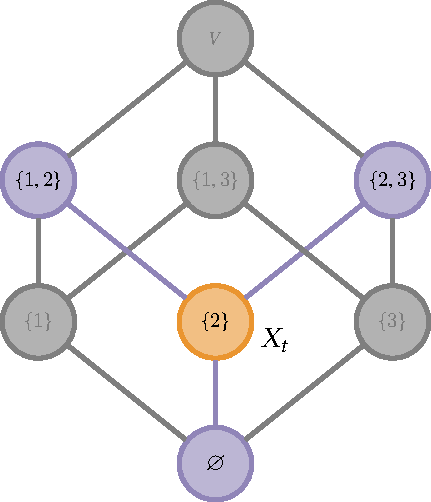
\includegraphics[width=0.55\textwidth]{figures/gibbs/lattice_gibbs_2.pdf}\\[1em]
\caption{An illustration of a single Gibbs step on ground set $V = \{1, 2, 3\}$, and current state $X_t = \{2\}$.
We first choose one of the neighbors of $X_t$ uniformly at random, and then either stay at $X_t$ or move to that neighbor according to the corresponding conditional probability.}
\label{fig:gibbs}
\end{figure}

The important thing to note here is that the computed conditional probabilities do not depend on the partition function $Z$, thus the chain can be simulated efficiently, even though $Z$ is unknown and hard to compute.
Moreover, it is easy to see that
\begin{align*}
\Delta_F(v \mid X_t) = \llbracket v\not\in X_t\rrbracket F(v \mid X_t) + \llbracket v\in X_t\rrbracket F(v \mid X_t\setminus\{v\}).
\end{align*}
Therefore, the sampler only requires a black box for the marginal gains of $F$, which are often faster to compute in practice than the values of $F$ itself.
Finally, it is easy to show that the stationary distribution of the chain constructed this way is $p$.

\section{Theoretical Results}
In the previous section we mentioned that exact computation of the partition function for the class of models we consider here is, in general, infeasible.
Only for very few exceptions, such as DPPs, is exact inference possible in polynomial time \cite{kulesza12}.
Even worse, it has been shown that the partition function of general Ising models is hard to approximate; in particular, there is no FPRAS for these models, unless RP = NP \cite{jerrum93}.
This implies that the mixing time of any Markov chain with such a stationary distribution will, in general, be exponential in $n$.
It is, therefore, our aim to derive sufficient conditions that guarantee sub-exponential mixing times for the general class of models.

In some of our results we will use the fact that any submodular function $F$ can be written as
\begin{align} \label{eq:decomp}
  F = c + m + f,
\end{align}
where $c \in \mathbb{R}$ is a constant that has no effect on distributions defined by \eqref{eq:pdef}; $m$ is a normalized ($m(\varnothing) = 0$) modular function; and $f$ is a normalized ($f(\varnothing) = 0$) monotone submodular function, that is, it additionally satisfies the monotonicity property $f(v|S) \geq 0$, for all $v \in V$, and all $S \subseteq V$.
A similar decomposition is possible for any supermodular function as well.


\subsection{Example: Log-submodular Grid}
To further highlight the hardness of inference in the general models we consider, we show that even for distributions defined through a seemingly benign subclass of submodular functions, mixing times can be exponential in $n$.
We say that a set function $F : 2^V \to \mathbb{R}$ is monotone, if $F(v|S) \geq 0$, for all $v \in V$, and all $S \subseteq V$.
Intuitively, adding elements to our set always leads to higher values.
\begin{lemma}
There is a family of monotone submodular functions $F_n$, such that, for the corresponding log-submodular family of distributions $p_n$ defined as in \eqref{eq:pdef}, the Metropolis chain has mixing time
\begin{align*}
  \tm  = \Omega(2^{n/2}),
\end{align*}
for any value of $\beta$.
\end{lemma}

\begin{proof}
The functions used to prove the above lemma are based on the following construction.
For any even $n \geq 2$, let $V_n = \{1,\ldots,n\}$, $R_n = \{1,\ldots,n/2\}$, and $C_n = \{n/2+1,\ldots,n\}$.
To define function $F_n : 2^{V_n} \to \mathbb{R}$, we conceptually use a $n/2 \times n/2$ square grid, whose rows are indexed by $R$ and columns by $C$.
Each cell $(i, j)$ of the grid is considered to be covered if either row $i \in R$ or column $j \in C$ is selected.
Formally, we define $F_n$ by
\begin{align*}
  F_n(S) = \frac{4}{n^2}\big\vert \sdef{(i, j) \in R \times C}{i \in S \lor j \in S}\big\vert,
\end{align*}
for any $S \subseteq V_n$, which results in $F_n(V_n) = 1$.

Assume a Metropolis chain with transition matrix $P$, and stationary distribution $p_n(S) \propto \exp(\beta F_n(S))$.
To prove a lower bound on the mixing time of this chain, we are going to upper bound the bottleneck ratio of set $T = \hat{R} \setminus \{V\}$, defined as
\begin{align*}
  \Phi(T) = \frac{Q(T, T^c)}{\pi(T)} = \frac{Q(T, \hat{C}) + Q(T, \hat{K})}{\pi(T)}.
\end{align*}

\begin{itemize}
  \item Computing $\pi(T)$:
    \begin{align*}
      \pi(T) &= |T| \frac{e^{\beta}}{Z} \tag*{by \eqref{eq:prop3}} \\
             &= (2^{n/2} - 1) \frac{e^{\beta}}{Z}. \tag*{by \eqref{eq:prop1}}
    \end{align*}
    Note that, by an analogous derivation, we get $\pi(\hat{C} \setminus \{V\}) = \pi(T)$ and, by \eqref{eq:prop2},
    \begin{align*}
      &\pi(T) + \pi(\hat{C} \setminus \{V\}) < 1 \\
      \Rightarrow\ \ &\pi(T) < 0.5.
    \end{align*}
  
  \item Computing $Q(T, \hat{C})$:
    \begin{align*}
      Q(T, \hat{C}) &= \sum_{x \in T} Q(x, \hat{C}) \\
                    &= \sum_{x \in T} Q(x, \{V\}) \tag*{by \eqref{eq:prop2}} \\
                    &= \sum_{x \in T} \frac{1}{2n} \frac{e^{\beta}}{Z} \tag*{by \eqref{eq:prop3}} \\
                    &= n \frac{1}{2n} \frac{e^{\beta}}{Z} = \frac{e^{\beta}}{2Z}.
    \end{align*}
    
  \item Computing $Q(T, \hat{K})$:
    \begin{align*}
      Q(T, \hat{K}) &= \sum_{x \in T} Q(x, \hat{K}) \\
                    &\leq \sum_{x \in T} \frac{1}{2n} \frac{e^{\beta - 4\beta/n^2}}{Z} \tag*{by \eqref{eq:prop4}} \\
                    &= \frac{2^{n/2} - 1}{2n} \frac{e^{\beta - 4\beta/n^2}}{Z}. \tag*{by \eqref{eq:prop1}}
    \end{align*}
\end{itemize}

Therefore, the bottleneck ratio can be bounded as follows:
\begin{align*}
  \Phi(T) &\leq \frac{1}{2^{n/2} - 1}\left(\frac{1}{2} + \frac{(2^{n/2} - 1) e^{-4\beta/n^2}}{2n}\right)\\
          &= \frac{1}{2(2^{n/2} - 1)} + \frac{e^{-4\beta/n^2}}{2n}.
\end{align*}

Using \citep[Theorem 7.3]{levin08book}, it follows that
\begin{align*}
  t_{mix}(1/4) \geq \frac{1}{4\Phi(T)} = \Omega(2^{n/2}).
\end{align*}

\newcommand{\subflen}{0.49\textwidth}
\newcommand{\scspacey}{0em}
\newcommand{\scspacex}{0em}
\begin{figure}[tb]
  \captionsetup[subfigure]{oneside,margin={2em,0em}}
  \begin{subfigure}[b]{\subflen}
	\centering
	\begin{tikzpicture}[
	%baseline,
	scale=1
	]
	\fill[blue!40!white] (-2,1) rectangle (2,2);
	\fill[blue!40!white] (-2,-1) rectangle (2,0);
	\fill[blue!40!white] (0,-2) rectangle (1,2);
	\draw[step=1cm,gray!80!black,line width=0.15em,line join=miter] (-2.01,-2.01) grid (2.01,2.01);
	
	\node at (-2.5,1.5) {\normalsize$1$};
	\node at (-2.5,0.5) {\normalsize$2$};
	\node at (-2.5,-0.5) {\normalsize$3$};
	\node at (-2.5,-1.5) {\normalsize$4$};
	\node at (-1.5,2.5) {\normalsize$5$};
	\node at (-0.5,2.5) {\normalsize$6$};
	\node at (0.5,2.5) {\normalsize$7$};
	\node at (1.5,2.5) {\normalsize$8$};
	\end{tikzpicture}
	%\caption{}
	\label{fig:grid}
  \end{subfigure}
  \begin{subfigure}[b]{\subflen}
  	\centering
    \trimbox{3em 6em 3em 6em}{
  	\begin{tikzpicture}[
  	%baseline,
  	scale=1,
    VN/.style={fill=white,draw=gray!80!black,circle,line width=0.15em,minimum size=1.5em},
    LL/.style={draw=gray!80!black,line width=0.1em}
    ]
    %\clip (-6,-4) rectangle (-6, -4);
    \draw [LL,fill=gray!30!white] (0,0) .. controls (4,4) and (4,-4) .. (0,0);
    \draw [LL,fill=gray!30!white] (0,0) .. controls (-4,4) and (-4,-4) .. (0,0);
    \node [VN] (V) at (0,0) {$V$};
    \node (R) at (-1.8, 0) {$\mathcal{R}$};
    \node (C) at (1.8, 0) {$\mathcal{C}$};
  	\end{tikzpicture}}
  	%\caption{}
  	\label{fig:ss}
  \end{subfigure}
  \caption{\emph{Left.} Example grid for $n = 8$ with the cells corresponding to $F_8(\{1,3,7\})$ shown shaded. \emph{Right.} Illustration of the state space and the bottleneck at $V$.}
\end{figure}

\end{proof}

\subsection{Polynomial-time mixing} \label{sect:poly}
Our guarantee for mixing times that are polynomial in $n$ depends crucially on the following quantity, which is defined for any set function $F : 2^V \to \mathbb{R}$:
\begin{align*}
  \zf \defeq \max_{A, B \subseteq V} \left|F(A) + F(B) - F(A \cup B) - F(A \cap B) \right|.
\end{align*}
Intuitively, $\zf$ quantifies a notion of distance to modularity.
To see this, note that a function $F$ is modular if and only if $F(A) + F(B) = F(A \cup B) + F(A \cap B)$, for all $A, B \subseteq V$.
For modular functions, therefore, we have $\zf = 0$.
Furthermore, a function $F$ is submodular if and only if $F(A) + F(B) \geq F(A \cup B) + F(A \cap B)$, for all $A, B \subseteq V$.
Similarly, $F$ is supermodular if the above holds with the sign reversed.
It follows that for submodular and supermodular functions, $\zf$ represents the worst-case amount by which $F$ violates the modular equality.
It is also important to note that, for submodular and supermodular functions, $\zf$ depends only on the monotone part of $F$; if we decompose $F$ according to \eqref{eq:decomp}, then it is easy to see that $\zf = \zeta_f$.
A trivial upper bound on $\zf$, therefore, is $\zf \leq f(V)$.
Another quantity that has been used in the past to quantify the deviation of a submodular function from modularity is the curvature \cite{conforti84}, defined as $\kappa_F \defeq 1 - \min_{v \in V} \left(F(v|V\setminus\{v\}) / F(v)\right)$.
Although of similar intuitive meaning, the multiplicative nature of its definition makes it significantly different from $\zf$, which is defined additively.

As an example of a function class with $\zf$ that do not depend on $n$, assume a ground set $V = \bigcup_{\ell = 1}^L V_{\ell}$, and consider functions $F(S) = \sum_{\ell = 1}^L \phi(|S \cap V_{\ell}|)$, where $\phi : \mathbb{R} \to \mathbb{R}$ is a bounded concave function, for example, $\phi(x) = \min\{\phi_{\max}, x\}$.
Functions of this form are submodular, and have been used in applications such as document summarization to encourage diversity \cite{lin11}.
It is easy to see that, for such functions, $\zf \leq L\phi_{\max}$, that is, $\zf$ is independent of $n$.

The following theorem establishes a bound on the mixing time of the Gibbs sampler run on models of the form \eqref{eq:pdef}.
The bound is exponential in $\zf$, but polynomial in $n$.
\begin{theorem} \label{thm:poly}
  For any function $F : 2^V \to \mathbb{R}$, the mixing time of the Gibbs sampler is bounded by
  \begin{align*}
    \tme \leq 2n^2 \exp(2 \beta \zf) \log\left(\frac{1}{\epsilon p_{\min}}\right),
  \end{align*}
  where $p_{\min} \defeq \displaystyle\min_{S \in \ss}p(S)$.
  If $F$ is submodular or supermodular, then the bound is improved to
  \begin{align*}
    \tme \leq 2n^2 \exp(\beta \zeta_f) \log\left(\frac{1}{\epsilon p_{\min}}\right).
  \end{align*}
\end{theorem}
Note that, since the factor of two that constitutes the difference between the two statements of the theorem lies in the exponent, it can have a significant impact on the above bounds.
The dependence on $p_{\min}$ is related to the (worst-case) starting state of the chain, and can be eliminated if we have a way to guarantee a high-probability starting state.
If $F$ is submodular or supermodular, this is usually straightforward to accomplish by using one of the standard constant-factor optimization algorithms \cite{nemhauser78,fujishige05} as a preprocessing step.
More generally, if $F$ is bounded by $0 \leq F(S) \leq F_{\max}$, for all $S \subseteq V$, then $\log (1/p_{\min}) = \mathcal{O}(n \beta F_{\max})$.

\paragraph{Canonical paths}
Our proof of \theoremref{thm:poly} is based on the method of \emph{canonical paths} \cite{jerrum03,sinclair92,jerrum89,diaconis91}.
The high-level idea of this method is to view the state space as a graph, and try to construct a path between each pair of states that carries a certain amount of flow specified by the stationary distribution under consideration.
Depending on the choice of these paths and the resulting load on the edges of the graph, we can derive bounds on the mixing time of the Markov chain.

More concretely, let us assume that for some set function $F$ and corresponding distribution $p$ as in \eqref{eq:pdef}, we construct the Gibbs chain on state space $\ss = 2^V$ with transition matrix $P$.
We can view the state space as a directed graph that has vertex set $\ss$, and for any $A, B \in \ss$, contains edge $(S, S')$ if and only if $S \sim S'$, that is, if and only if $S$ and $S'$ differ by exactly one element.
Now, assume that, for any pair of states $A, B \in \ss$, we define what is called a canonical path $\gamma_{AB} \defeq (A = S_0, S_1, \ldots, S_{\ell} = B)$, such that all $(S_i, S_{i+1})$ are edges in the above graph.
We denote the length of path $\gamma_{AB}$ by $|\gamma_{AB}|$, and define $Q(S, S') \defeq p(S) P(S, S')$.
We also denote the set of all pairs of states whose canonical path goes through $(S, S')$ by $\mathcal{C}_{SS'} \defeq \sdef{(A, B) \in \ss \times \ss}{(S, S') \in \gamma_{AB}}$.
The following quantity, referred to as the \emph{congestion} of an edge, uses a collection of canonical paths to quantify to what amount that edge is overloaded:
\begin{align} \label{eq:cong}
  \rho(S, S') \defeq \frac{1}{Q(S, S')} \sum_{(A, B) \in \mathcal{C}_{SS'}} p(A) p(B) |\gamma_{AB}|.
\end{align}
The denominator $Q(S, S')$ quantifies the capacity of edge $(S, S')$, while the sum represents the total flow through that edge according to the choice of canonical paths.
The congestion of the whole graph is then defined as $\rho \defeq \max_{S \sim S'}\rho(S, S')$.
Low congestion implies that there are no bottlenecks in the state space, and the chain can move around fast, which also suggests rapid mixing.
The following theorem makes this concrete.

\begin{theorem}[\hspace{1sp}\cite{sinclair92,jerrum03}] \label{thm:cpath}
  For any collection of canonical paths with congestion $\rho$, the mixing time of the chain is bounded by
  \begin{align*}
  	\tme \leq \rho \log\left(\frac{1}{\epsilon p_{\mathrm{min}}}\right).
  \end{align*}
%  where $p_{\min} \defeq \displaystyle\min_{S \in \ss}p(S)$.
\end{theorem}

\paragraph{Proof outline of \theoremref{thm:poly}}
To apply \theoremref{thm:cpath} to our class of distributions, we need to construct a set of canonical paths in the corresponding state space $2^V$, and upper bound the resulting congestion.
First, note that, to transition from state $A \in \ss$ to state $B \in \ss$, in our case, it is enough to remove the elements of $A \setminus B$ and add the elements of $B \setminus A$.
Each removal and addition corresponds to an edge in the state space graph, and the order of these operations identify a canonical path in this graph that connects $A$ to $B$.
For our analysis, we assume a fixed order on $V$ (e.g., the natural order of the elements themselves), and perform the operations according to this order.

Having defined the set of canonical paths, we proceed to bounding the congestion $\rho(S, S')$ for any edge $(S, S')$.
The main difficulty in bounding $\rho(S, S')$ is due to the sum in \eqref{eq:cong} over all pairs in $\mathcal{C}_{SS'}$.
To simplify this sum we construct for each edge $(S, S')$ an injective map $\ess : \mathcal{C}_{SS'} \to \ss$; this is a combinatorial encoding technique that has been previously used in similar proofs to ours \cite{jerrum03}.
We then prove the following key lemma about these maps.

\begin{lemma} \label{lem:poly}
  For any $S \sim S'$, and any $A, B \in \ss$, it holds that
  \begin{align*}
  	p(A)p(B) \leq 2n\exp(2 \beta \zf)Q(S, S')p(\ess(A, B)).
  \end{align*}
\end{lemma}

Since $\ess$ is injective, it follows that $\sum_{(A, B) \in \mathcal{C}_{SS'}} p(\ess(A, B)) \leq 1$.
Furthermore, it is clear that each canonical path $\gamma_{AB}$ has length $|\gamma_{AB}| \leq n$, since we need to add and/or remove at most $n$ elements to get from state $A$ to state $B$.
Combining these two facts with the above lemma, we get
\begin{align*}
  \rho(S, S') \leq 2n^2 \exp(2 \beta \zf).
\end{align*}
If $F$ is submodular or supermodular, we show that the dependence on $\zf$ in \lemmaref{lem:poly}  is improved to $\exp(\beta \zf)$.
More details can be found in the longer version of the paper.

\subsection{Fast mixing}
We now proceed to show that, under some stronger conditions, we are able to establish even faster---$\mathcal{O}(n \log n)$---mixing.
For any function $F$, we denote $\D_F(v|S) \defeq F(S \cup \{v\}) - F(S \setminus \{v\})$, and define the following quantity,
\begin{align*}
  \gf &\defeq \max_{\substack{S \subseteq V\\r \in V}} \sum_{\substack{v \in V}} \tanh\left(\frac{\beta}{2} \big|\D_F(v|S) - \D_F(v|S \cup \{r\})\big| \right),
\end{align*}

which quantifies the (maximum) total influence of an element $r \in V$ on the values of $F$.
For example, if the inclusion of $r$ makes no difference with respect to other elements of the ground set, we will have $\gf = 0$.
The following theorem establishes conditions for fast mixing of the Gibbs sampler when run on models of the form \eqref{eq:pdef}.

\begin{theorem} \label{thm:fast}
  For any set function $F : 2^V \to \mathbb{R}$, if $\gf < 1$, then the mixing time of the Gibbs sampler is bounded by
  \begin{align*}
  	\tme \leq \frac{1}{1 - \gf}n(\log n + \log \frac{1}{\epsilon}).
  \end{align*}
  If $F$ is additionally submodular or supermodular, and is decomposed according to \eqref{eq:decomp}, then
  \begin{align*}
  	\tme \leq \frac{1}{1 - \gsf}n(\log n + \log \frac{1}{\epsilon}).
  \end{align*}
\end{theorem}
Note that, in the second part of the theorem, $\gsf$ depends only on the monotone part of $F$. 
We have seen in \sectref{sect:setup} that some commonly used models are based on decomposable functions that can be written in the form \eqref{eq:fdec}.
We prove the following corollary that provides an easy to check condition for fast mixing of the Gibbs sampler when $F$ is a decomposable submodular function.

\begin{cor} \label{cor:fast}
  For any submodular function $F$ that can be written in the form of \eqref{eq:fdec}, with $f$ being its monotone (also decomposable) part according to \eqref{eq:decomp}, if we define
  \begin{align*}
  	\theta_f \defeq \max_{v \in V} \sum_{\ell \in [L]} \sqrt{f_{\ell}(v)} \hspace{1em}\textrm{and}\hspace{1em} \lambda_f \defeq \max_{\ell \in [L]} \sum_{v \in V} \sqrt{f_{\ell}(v)},
  \end{align*}
  then it holds that
  \begin{align*}
  	\gsf \leq \frac{\beta}{2} \theta_f \lambda_f.
  \end{align*}
\end{cor}

For example, applying this to the facility location model defined in \sectref{sect:setup}, we get $\theta_f = \max_{v} \sum_{\ell = 1}^L \sqrt{w_{v, \ell}}$, and $\lambda_f = \max_{\ell} \sum_{v \in V} \sqrt{w_{v, \ell}}$, and obtain fast mixing if $\theta_f \lambda_f \leq 2/\beta$.
As a special case, if we consider the class of set cover functions ($w_{v, \ell} \in \{0, 1\}$), such that each $v \in V$ covers at most $\delta$ sets, and each set $\ell \in [L]$ is covered by at most $\delta$ elements, then $\theta_f, \lambda_f \leq \delta$, and we obtain fast mixing if $\delta^2 \leq 2/\beta$.
Note, that the corollary can be trivially applied to any submodular function by taking $L=1$, but may, in general, result in a loose bound if used that way.

\paragraph{Coupling}
Our proof of \theoremref{thm:fast} is based on the \emph{coupling} technique \cite{aldous83}; more specifically, we use the \emph{path coupling} method \cite{bubley97,levin08,jerrum03}.
Given a Markov chain $(X_t)$ on state space $\ss$ with transition matrix $P$, a coupling for $(Z_t)$ is a new Markov chain $(X_t, Y_t)$ on state space $\ss \times \ss$, such that both $(X_t)$ and $(Y_t)$ are by themselves Markov chains with transition matrix $P$.
The idea is to construct the coupling in such a way that, even when the starting points $X_0$ and $Y_0$ are different, the chains $(X_t)$ and $(Y_t)$ tend to coalesce.
Then, it can be shown that the coupling time $t_{\mathrm{couple}} \defeq \min\sdef{t \geq 0}{X_t = Y_t}$ is closely related to the mixing time of the original chain $(Z_t)$. \cite{levin08}

The main difficulty in applying the coupling approach lies in the construction of the coupling itself, for which one needs to consider any possible pair of states $(Y_t, Z_t)$.
The path coupling technique makes this construction easier by utilizing the same state-space graph that we used to define canonical paths in \sectref{sect:poly}.
The core idea is to first define a coupling only over adjacent states, and then extend it for any pair of states by using a metric on the graph.
More concretely, let us denote by $d : \ss \times \ss \to \mathbb{R}$ the \emph{path metric} on state space $\ss$; that is, for any $x, y \in \ss$, $d(x, y)$ is the minimum length of any path from $x$ to $y$ in the state space graph.
The following theorem establishes fast mixing using this metric, as well as the diameter of the state space, $\mathrm{diam}(\ss) \defeq \max_{x,y \in \ss}d(x, y)$.
\begin{theorem}[\hspace{1sp}\cite{bubley97,levin08}] \label{thm:pc}
For any Markov chain $(Z_t)$, if $(X_t, Y_t)$ is a coupling, such that, for some $a \geq 0$, and any $x, y \in \ss$ with $x \sim y$, it holds that
\begin{align*}
  \E[d(X_{t+1}, Y_{t+1}) \mid X_t = x, Y_t = y] \leq e^{-\alpha}d(x, y),
\end{align*}
then the mixing time of the original chain is bounded by
\begin{align*}
  \tme \leq \frac{1}{\alpha}\left(\log(\mathrm{diam}(\ss)) + \log\frac{1}{\epsilon} \right).
\end{align*}
\end{theorem}

\paragraph{Proof outline of \theoremref{thm:fast}}
In our case, the path metric $d$ is the Hamming distance between the binary vectors representing the states (equivalently, the number of elements by which two sets differ).
We need to construct a suitable coupling $(X_t, Y_t)$ for any pair of states $x \sim y$.
Consider the two corresponding sets $S, R \subseteq V$ that differ by exactly one element, and assume that $R = S \cup \{r\}$, for some $r \in V$. (The case $S = R \cup \{s\}$ for some $s \in V$ is completely analogous.)
Remember that the Gibbs sampler first chooses an element $v \in V$ uniformly at random, and then adds or removes it according to the conditional probabilities.
Our goal is to make the same updates happen to both $S$ and $R$ as frequently as possible.
As a first step, we couple the candidate element for update $v \in V$ to always be the same in both chains.
Then, we have to distinguish between the following cases.

If $v = r$, then the conditionals for both chains are identical, therefore we can couple both chains to add $r$ with probability $p_{\mathrm{add}} \defeq p(S \cup \{r\}) / (p(S) + p(S \cup \{r\}))$, which will result in new sets $S' = R' = S \cup \{r\}$, or remove $r$ with probability $1 - p_{\mathrm{add}}$, which will result in new sets $S' = R' = S$.
Either way, we will have $d(S', R') = 0$.
  
If $v \neq r$, we cannot always couple the updates of the chains, because the conditional probabilities of the updates are different.
In fact, we are forced to have different updates (one chain adding $v$, the other chain removing $v$) with probability equal to the difference of the corresponding conditionals, which we denote here by $p_{\mathrm{dif}}(v)$.
%  \begin{align*}
%  	p_{\mathrm{dif}}(v) \defeq \left|\frac{p(S \cup \{v\})}{p(S \cup \{v\}) + p(S \setminus \{v\})} - \frac{p(R \cup \{v\})}{p(R \cup \{v\}) + p(R \setminus \{v\})}\right|.
%  \end{align*}
If this is the case, we will have $d(S', R') = 2$, otherwise the chains will make the same update and will still differ only by element $r$, that is, $d(S', R') = 1$.
  
Putting together all the above, we get the following expected distance after one step:
\begin{align*}
  \E[d(S', R')] = 1 -\frac{1}{n} + \frac{1}{n}\sum_{v \neq r}p_{\mathrm{dif}}(v) \leq 1 - \frac{1}{n}(1 - \gf) \leq \exp\left(-\frac{1-\gf}{n}\right).
\end{align*}
Our result follows from applying \theoremref{thm:pc} with $\alpha = \gf/n$, noting that $\mathrm{diam}(\ss) = n$.

\section{Experiments}
We compare the Gibbs sampler against the variational approach proposed by Djolonga and Krause \cite{djolonga14} for performing inference in models of the form \eqref{eq:pdef}, and use the same three models as in their experiments.
We briefly review here the experimental setup and refer to their paper for more details.

The first is a (log-submodular) facility location model with an added modular term that penalizes the number of selected elements, that is, $p(S) \propto \exp(F(S)-2|S|)$, where $F$ is a submodular facility location function.
The model is constructed from randomly subsampling real data from a problem of sensor placement in a water distribution network \cite{krause08}.
In the experiments, we iteratively condition on random observations for each variable in the ground set.
The second is a (log-supermodular) pairwise Markov random field (MRF; a generalized Ising model with varying weights), constructed by first randomly sampling points from a 2-D two-cluster Gaussian mixture model, and then introducing a pairwise potential for each pair of points with exponentially-decreasing weight in the distance of the pair.
In the experiments, we iteratively condition on pairs of observations, one from each cluster.
The third is a (log-supermodular) higher-order MRF, which is constructed by first generating a random Watts-Strogatz graph, and then creating one higher-order potential per node, which contains that node and all of its neighbors in the graph.
The strength of the potentials is controlled by a parameter $\mu$, which is closely related to the curvature of the functions that define them.
In the experiments, we vary this parameter from $0$ (modular model) to $1$ (``strongly'' supermodular model).

For all three models, we constrain the size of the ground set to $n = 20$, so that we are able to compute, and compare against, the exact marginals.
Furthermore, we run multiple repetitions for each model to account for the randomness of the model instance, and the random initialization of the Gibbs sampler.
The marginals we compute are of the form $p(v \in S \mid C \subseteq S \subseteq D)$, for all $v \in V$.
We run the Gibbs sampler for $100$, $500$, and $2000$ iterations on each problem instance.
In compliance with recommended MCMC practice \cite{gelman11}, we discard the first half of the obtained samples as burn-in, and only use the second half for estimating the marginals.

\figref{fig:exp} compares the average absolute error of the approximate marginals with respect to the exact ones.
The averaging is performed over $v \in V$, and over the different repetitions of each experiment; errorbars depict two standard errors.
The two variational approximations are obtained from factorized distributions associated with modular lower and upper bounds respectively \cite{djolonga14}.
We notice a similar trend on all three models.
For the regimes that correspond to less ``peaked'' posterior distributions (small number of conditioned variables, small $\mu$), even $100$ Gibbs iterations outperform both variational approximations.
The latter gain an advantage when the posterior is concentrated around only a few states, which happens after having conditioned on almost all variables in the first two models, or for $\mu$ close to $1$ in the third model.

\setlength\figureheight{0.45\textwidth}
\setlength\figurewidth{0.7\textwidth}
\newcommand{\subflen}{\textwidth}
\begin{figure}[tb]
  \captionsetup[subfigure]{oneside,margin={2em,0em}}
  \begin{subfigure}[b]{\subflen}
    \centering
    \begin{tikzpicture}

\begin{axis}[%
tick label style={/pgf/number format/fixed,font=\sffamily\small},
label style={font=\sffamily\small},
legend style={font=\sffamily\small},
view={0}{90},
width=\figurewidth,
height=\figureheight,
xmin=0, xmax=19.5,
xtick={0, 2, 4, 6, 8, 10, 12, 14, 16, 18},
xticklabels={0, 2, 4, 6, 8, 10, 12, 14, 16, 18},
ytick={0, 0.05, 0.1, 0.15, 0.2},
yticklabels={0, 0.05, 0.1, 0.15, 0.2},
xlabel={Number of conditioned elements},
xlabel shift=0em,
ymin=0, ymax=0.2,
ylabel={Abs. marginal error},
ylabel shift=0em,
major tick length=2pt,
axis lines*=left,
legend cell align=left,
clip=false,
legend style={anchor=east,at={(1.4,0.5)},draw=none,row sep=0},
every axis plot/.append style={
  mark=*,
  mark options={solid},
  mark size=1.7pt,
  line width=1.2pt,
  opacity=0.9,
}
]

\addplot [
color=col2,
densely dashed,
error bars/.cd,
error bar style={solid, line width=1pt},
y dir=both,
y explicit
]
coordinates{
(0,0.10663)+-(0.00557,0.00557)(1,0.10204)+-(0.00556,0.00556)(2,0.09616)+-(0.00573,0.00573)(3,0.09341)+-(0.00622,0.00622)(4,0.08953)+-(0.00630,0.00630)(5,0.08529)+-(0.00617,0.00617)(6,0.07930)+-(0.00668,0.00668)(7,0.07646)+-(0.00701,0.00701)(8,0.07102)+-(0.00678,0.00678)(9,0.06403)+-(0.00686,0.00686)(10,0.05621)+-(0.00724,0.00724)(11,0.05193)+-(0.00752,0.00752)(12,0.04229)+-(0.00756,0.00756)(13,0.04054)+-(0.00800,0.00800)(14,0.03328)+-(0.00798,0.00798)(15,0.02909)+-(0.00816,0.00816)(16,0.02200)+-(0.00831,0.00831)(17,0.01509)+-(0.00851,0.00851)(18,0.00992)+-(0.00832,0.00832)(19,0.00000)+-(0.00000,0.00000)

};
\addlegendentry{Var (upper)}

\addplot [
color=col3,
densely dashed,
error bars/.cd,
error bar style={solid, line width=1pt},
y dir=both,
y explicit
]
coordinates{
(0,0.07810)+-(0.00588,0.00588)(1,0.07520)+-(0.00588,0.00588)(2,0.06963)+-(0.00574,0.00574)(3,0.06618)+-(0.00581,0.00581)(4,0.06380)+-(0.00573,0.00573)(5,0.06017)+-(0.00570,0.00570)(6,0.05563)+-(0.00590,0.00590)(7,0.05454)+-(0.00632,0.00632)(8,0.05097)+-(0.00601,0.00601)(9,0.04707)+-(0.00629,0.00629)(10,0.04101)+-(0.00624,0.00624)(11,0.03708)+-(0.00622,0.00622)(12,0.03014)+-(0.00596,0.00596)(13,0.02921)+-(0.00646,0.00646)(14,0.02411)+-(0.00624,0.00624)(15,0.02133)+-(0.00643,0.00643)(16,0.01586)+-(0.00636,0.00636)(17,0.01066)+-(0.00618,0.00618)(18,0.00642)+-(0.00509,0.00509)(19,0.00000)+-(0.00000,0.00000)

};
\addlegendentry{Var (lower)}

\addplot [
color=col1,
error bars/.cd,
error bar style={line width=1pt},
y dir=both,
y explicit
]
coordinates{
(0,0.18132)+-(0.00775,0.00775)(1,0.18311)+-(0.00711,0.00711)(2,0.17703)+-(0.00781,0.00781)(3,0.16580)+-(0.00758,0.00758)(4,0.16179)+-(0.00787,0.00787)(5,0.16001)+-(0.00801,0.00801)(6,0.15211)+-(0.00744,0.00744)(7,0.13779)+-(0.00673,0.00673)(8,0.14007)+-(0.00832,0.00832)(9,0.13122)+-(0.00748,0.00748)(10,0.12540)+-(0.00707,0.00707)(11,0.11669)+-(0.00804,0.00804)(12,0.10816)+-(0.00724,0.00724)(13,0.10136)+-(0.00767,0.00767)(14,0.09844)+-(0.00764,0.00764)(15,0.08261)+-(0.00646,0.00646)(16,0.08397)+-(0.00875,0.00875)(17,0.06379)+-(0.00613,0.00613)(18,0.05179)+-(0.00584,0.00584)(19,0.03074)+-(0.00525,0.00525)

};
\addlegendentry{Gibbs (200)}

\addplot [
color=col1!70!black,
error bars/.cd,
error bar style={line width=1pt},
y dir=both,
y explicit
]
coordinates{
(0,0.09306)+-(0.00439,0.00439)(1,0.09202)+-(0.00361,0.00361)(2,0.08977)+-(0.00423,0.00423)(3,0.08553)+-(0.00440,0.00440)(4,0.08069)+-(0.00420,0.00420)(5,0.07967)+-(0.00410,0.00410)(6,0.07670)+-(0.00386,0.00386)(7,0.07411)+-(0.00426,0.00426)(8,0.06926)+-(0.00421,0.00421)(9,0.06386)+-(0.00374,0.00374)(10,0.05764)+-(0.00364,0.00364)(11,0.05508)+-(0.00342,0.00342)(12,0.05165)+-(0.00340,0.00340)(13,0.04912)+-(0.00426,0.00426)(14,0.04226)+-(0.00354,0.00354)(15,0.03888)+-(0.00346,0.00346)(16,0.03193)+-(0.00262,0.00262)(17,0.02857)+-(0.00321,0.00321)(18,0.02136)+-(0.00255,0.00255)(19,0.01238)+-(0.00209,0.00209)

};
\addlegendentry{Gibbs (1000)}

\addplot [
color=col1!40!black,
error bars/.cd,
error bar style={line width=1pt},
y dir=both,
y explicit
]
coordinates{
(0,0.04322)+-(0.00211,0.00211)(1,0.04114)+-(0.00199,0.00199)(2,0.03940)+-(0.00203,0.00203)(3,0.03887)+-(0.00181,0.00181)(4,0.03745)+-(0.00172,0.00172)(5,0.03510)+-(0.00205,0.00205)(6,0.03227)+-(0.00155,0.00155)(7,0.03289)+-(0.00159,0.00159)(8,0.03000)+-(0.00154,0.00154)(9,0.03004)+-(0.00180,0.00180)(10,0.02638)+-(0.00186,0.00186)(11,0.02532)+-(0.00192,0.00192)(12,0.02375)+-(0.00167,0.00167)(13,0.02039)+-(0.00154,0.00154)(14,0.01933)+-(0.00133,0.00133)(15,0.01802)+-(0.00170,0.00170)(16,0.01410)+-(0.00123,0.00123)(17,0.01285)+-(0.00133,0.00133)(18,0.01019)+-(0.00116,0.00116)(19,0.00610)+-(0.00103,0.00103)

};
\addlegendentry{Gibbs (5000)}

\end{axis}
\end{tikzpicture}
    \caption{Facility location}
    \label{fig:exp1}
  \end{subfigure}\\[1em]
  \begin{subfigure}[b]{\subflen}
    \centering
    \begin{tikzpicture}

\begin{axis}[%
tick label style={/pgf/number format/fixed,font=\sffamily\small},
label style={font=\sffamily\small},
legend style={font=\sffamily\small},
view={0}{90},
width=\figurewidth,
height=\figureheight,
xmin=0, xmax=9,
xtick={0, 1, 2, 3, 4, 5, 6, 7, 8, 9},
xticklabels={0, 1, 2, 3, 4, 5, 6, 7, 8, 9},
xlabel={Number of conditioned pairs},
xlabel shift=0em,
ytick={0, 0.1, 0.2, 0.3, 0.4},
yticklabels={0, 0.1, 0.2, 0.3, 0.4},
ymin=0, ymax=0.4,
ylabel={Abs. marginal error},
ylabel shift=0em,
tick label style={/pgf/number format/fixed,font=\sffamily},
major tick length=2pt,
axis lines*=left,
legend cell align=left,
clip=false,
legend style={anchor=east,at={(1.4,0.5)},draw=none,row sep=0},
every axis plot/.append style={
  mark=*,
  mark options={solid},
  mark size=1.7pt,
  line width=1.2pt,
  opacity=0.9,
}
]

\addplot [
color=gcol2,
densely dashed,
error bars/.cd,
error bar style={solid, line width=1pt},
y dir=both,
y explicit
]
coordinates{
(0,0.00000)+-(0.00000,0.00000)(1,0.13529)+-(0.00946,0.00946)(2,0.15721)+-(0.00700,0.00700)(3,0.13708)+-(0.00529,0.00529)(4,0.10985)+-(0.00407,0.00407)(5,0.08099)+-(0.00343,0.00343)(6,0.05466)+-(0.00307,0.00307)(7,0.03219)+-(0.00203,0.00203)(8,0.01434)+-(0.00163,0.00163)(9,0.00002)+-(0.00001,0.00001)

};
\addlegendentry{Var (upper)}

\addplot [
color=gcol3,
densely dashed,
error bars/.cd,
error bar style={solid, line width=1pt},
y dir=both,
y explicit
]
coordinates{
(0,0.37813)+-(0.00543,0.00543)(1,0.18469)+-(0.00939,0.00939)(2,0.10135)+-(0.00621,0.00621)(3,0.06615)+-(0.00459,0.00459)(4,0.04468)+-(0.00314,0.00314)(5,0.03022)+-(0.00218,0.00218)(6,0.01988)+-(0.00164,0.00164)(7,0.01247)+-(0.00134,0.00134)(8,0.00556)+-(0.00096,0.00096)(9,0.00004)+-(0.00002,0.00002)

};
\addlegendentry{Var (lower)}

\addplot [
color=gcol1!50!white,
error bars/.cd,
error bar style={line width=1pt},
y dir=both,
y explicit
]
coordinates{
(0,0.33633)+-(0.01046,0.01046)(1,0.26388)+-(0.01602,0.01602)(2,0.20123)+-(0.01784,0.01784)(3,0.15406)+-(0.00906,0.00906)(4,0.13772)+-(0.00710,0.00710)(5,0.10925)+-(0.00641,0.00641)(6,0.10391)+-(0.00728,0.00728)(7,0.08370)+-(0.00673,0.00673)(8,0.06571)+-(0.00576,0.00576)(9,0.04372)+-(0.00535,0.00535)

};
\addlegendentry{Gibbs (200)}

\addplot [
color=gcol1,
error bars/.cd,
error bar style={line width=1pt},
y dir=both,
y explicit
]
coordinates{
(0,0.21841)+-(0.01672,0.01672)(1,0.14267)+-(0.01358,0.01358)(2,0.09997)+-(0.00997,0.00997)(3,0.07768)+-(0.00569,0.00569)(4,0.06026)+-(0.00361,0.00361)(5,0.05201)+-(0.00301,0.00301)(6,0.04489)+-(0.00266,0.00266)(7,0.03743)+-(0.00248,0.00248)(8,0.02995)+-(0.00245,0.00245)(9,0.01929)+-(0.00241,0.00241)

};
\addlegendentry{Gibbs (1000)}

\addplot [
color=gcol1!50!black,
error bars/.cd,
error bar style={line width=1pt},
y dir=both,
y explicit
]
coordinates{
(0,0.11321)+-(0.01234,0.01234)(1,0.07095)+-(0.00618,0.00618)(2,0.04435)+-(0.00305,0.00305)(3,0.03288)+-(0.00182,0.00182)(4,0.02745)+-(0.00137,0.00137)(5,0.02488)+-(0.00146,0.00146)(6,0.02025)+-(0.00146,0.00146)(7,0.01715)+-(0.00121,0.00121)(8,0.01316)+-(0.00107,0.00107)(9,0.00884)+-(0.00088,0.00088)

};
\addlegendentry{Gibbs (5000)}

\end{axis}
\end{tikzpicture}
    \caption{Pairwise MRF}
    \label{fig:exp2}
  \end{subfigure}\\[1em]
  \begin{subfigure}[b]{\subflen}
    \centering
    \begin{tikzpicture}

\begin{axis}[%
tick label style={/pgf/number format/fixed,font=\sffamily\small},
label style={font=\sffamily\small},
legend style={font=\sffamily\small},
view={0}{90},
width=\figurewidth,
height=\figureheight,
xmin=0, xmax=1,
xtick={0, 0.2, 0.4, 0.6, 0.8, 1},
xticklabels={0, 0.2, 0.4, 0.6, 0.8, 1},
xlabel={$\mu$},
xlabel shift=0em,
ymin=0, ymax=0.15,
ytick={0, 0.05, 0.1, 0.15},
yticklabels={0, 0.05, 0.1, 0.15},
ylabel={Abs. marginal error},
ylabel shift=0em,
major tick length=2pt,
axis lines*=left,
legend cell align=left,
clip=false,
legend style={anchor=east,at={(1.4,0.5)},draw=none,row sep=0},
every axis plot/.append style={
  mark=*,
  mark options={solid},
  mark size=1.7pt,
  line width=1.2pt,
  opacity=0.9,
}
]

\addplot [
color=gcol2,
densely dashed,
error bars/.cd,
error bar style={solid, line width=1pt},
y dir=both,
y explicit
]
coordinates{
(0.01,0.07265)+-(0.00221,0.00221)(0.1189,0.06349)+-(0.00165,0.00165)(0.2278,0.05363)+-(0.00108,0.00108)(0.3367,0.04434)+-(0.00060,0.00060)(0.4456,0.03578)+-(0.00055,0.00055)((0.5544,0.02734)+-(0.00053,0.00053)(0.6633,0.02009)+-(0.00046,0.00046)(0.7722,0.01307)+-(0.00034,0.00034)(0.8811,0.00630)+-(0.00017,0.00017)(0.99,0.00050)+-(0.00002,0.00002)

};
\addlegendentry{Var (upper)}

\addplot [
color=gcol3,
densely dashed,
error bars/.cd,
error bar style={solid, line width=1pt},
y dir=both,
y explicit
]
coordinates{
(0.01,0.04309)+-(0.00738,0.00738)(0.1189,0.04162)+-(0.00706,0.00706)(0.2278,0.03337)+-(0.00505,0.00505)(0.3367,0.03534)+-(0.00472,0.00472)(0.4456,0.02535)+-(0.00388,0.00388)(0.5544,0.02088)+-(0.00247,0.00247)(0.6633,0.01532)+-(0.00153,0.00153)(0.7722,0.01047)+-(0.00126,0.00126)(0.8811,0.00547)+-(0.00054,0.00054)(0.99,0.00044)+-(0.00004,0.00004)

};
\addlegendentry{Var (lower)}

\addplot [
color=gcol1!50!white,
error bars/.cd,
error bar style={line width=1pt},
y dir=both,
y explicit
]
coordinates{
(0.01,0.08946)+-(0.01131,0.01131)(0.1189,0.09087)+-(0.00957,0.00957)(0.2278,0.09140)+-(0.00838,0.00838)(0.3367,0.09382)+-(0.00739,0.00739)(0.4456,0.09379)+-(0.00741,0.00741)(0.5544,0.10270)+-(0.00759,0.00759)(0.6633,0.11009)+-(0.00709,0.00709)(0.7722,0.10570)+-(0.00735,0.00735)(0.8811,0.10047)+-(0.00579,0.00579)(0.99,0.11209)+-(0.00756,0.00756)

};
\addlegendentry{Gibbs (200)}

\addplot [
color=gcol1,
error bars/.cd,
error bar style={line width=1pt},
y dir=both,
y explicit
]
coordinates{
(0.01,0.04593)+-(0.00491,0.00491)(0.1189,0.04659)+-(0.00466,0.00466)(0.2278,0.04902)+-(0.00465,0.00465)(0.3367,0.05229)+-(0.00452,0.00452)(0.4456,0.05153)+-(0.00349,0.00349)(0.5544,0.05246)+-(0.00351,0.00351)(0.6633,0.05408)+-(0.00386,0.00386)(0.7722,0.05374)+-(0.00316,0.00316)(0.8811,0.05628)+-(0.00312,0.00312)(0.99,0.05585)+-(0.00313,0.00313)

};
\addlegendentry{Gibbs (1000)}

\addplot [
color=gcol1!50!black,
error bars/.cd,
error bar style={line width=1pt},
y dir=both,
y explicit
]
coordinates{
(0.01,0.02303)+-(0.00238,0.00238)(0.1189,0.02210)+-(0.00170,0.00170)(0.2278,0.02145)+-(0.00192,0.00192)(0.3367,0.02355)+-(0.00190,0.00190)(0.4456,0.02305)+-(0.00171,0.00171)(0.5544,0.02423)+-(0.00148,0.00148)(0.6633,0.02533)+-(0.00155,0.00155)(0.7722,0.02373)+-(0.00120,0.00120)(0.8811,0.02506)+-(0.00162,0.00162)(0.99,0.02563)+-(0.00157,0.00157)

};
\addlegendentry{Gibbs (5000)}

\end{axis}
\end{tikzpicture}
    \caption{Higher-order MRF}
    \label{fig:exp3}
  \end{subfigure}
  \caption{Absolute error of the marginals computed by the Gibbs sampler compared to variational inference \cite{djolonga14}.
  	A modest $500$ Gibbs iterations outperform the variational method for the most part.}
  \label{fig:exp}
\end{figure}


\paragraph{Related Work.}
In contemporary work to ours, Rebeschini and Karbasi \cite{rebeschini15} analyzed the mixing times of log-submodular models.
Using a method based on matrix norms, which was previously introduced by Dyer et al. \cite{dyer09}, and is closely related to path coupling, they arrive at a similar---though not directly comparable---condition to the one we presented in \theoremref{thm:fast}.

Iyer and Bilmes \cite{iyer15} recently considered a different class of probabilistic models, called submodular point processes, which are also defined through submodular functions, and have the form $p(S) \propto F(S)$.
They showed that inference in SPPs is, in general, also a hard problem, and provided approximations and closed-form solutions for some subclasses.

The canonical path method for bounding mixing times has been previously used in applications, such as approximating the partition function of ferromagnetic Ising models \cite{jerrum93}, approximating matrix permanents \cite{jerrum89,jerrum04perm}, and counting matchings in graphs \cite{jerrum03}.
The most prominent application of coupling-based methods is counting $k$-colorings in low-degree graphs \cite{jerrum95,bubley98,jerrum03}.
Other applications include counting independent sets in graphs \cite{dyer00}, and approximating the partition function of various subclasses of Ising models at high temperatures \cite{levin08}.

\todo{Add Chengtao constrained etc. paper}
\todo{Add DPP -- Rayleigh papers}


\section{Conclusion}
We considered the problem of performing marginal inference using MCMC sampling techniques in probabilistic models defined through submodular functions.
In particular, we presented for the first time sufficient conditions to obtain upper bounds on the mixing time of the Gibbs sampler in general log-submodular and log-supermodular models.
Furthermore, we demonstrated that, in practice, the Gibbs sampler compares favorably to previously proposed variational approximations, at least in regimes of high uncertainty.
We believe that this is an important step towards a unified framework for further analysis and practical application of this rich class of probabilistic submodular models.